\documentclass{../praktikum-ppt}
\usepackage[simplified]{pgf-umlcd}

\author[Tew \& Haf]{Teosofi Hidayah Agung \\ Hafidz Mulia}
\date{28 April 2025}
\title[Alpro 2 - Week 5]{\textit{Class} \& \textit{Object}}
\institute[Matematika ITS]{Departemen Matematika\\ Institut Teknologi Sepuluh Nopember}

\begin{document}

{\usebackgroundtemplate{
  \tikz[overlay,remember picture] \node[opacity=0.2, at=(current page.center)]{
\includegraphics[width=\paperwidth]{bg_22}};}
\begin{frame}
  \titlepage
\end{frame}
}

\AtBeginSection{
    {\usebackgroundtemplate{
     \tikz[overlay,remember picture] \node[opacity=0.1, at=(current page.center)]{
\includegraphics[width=\paperwidth]{code_bg}};}
    \begin{frame}{Daftar isi}
        \tableofcontents[currentsection]
        % \begin{tikzpicture}[overlay, remember picture] 
        %     \node at ([yshift=.5cm]current page.south east) [
        %         anchor = south east, 
        %         ] {
        %     \animategraphics[autoplay,loop,width=0.2\textwidth]{30}{Arisu Dance/Arisu Dance-}{0}{186}
        %     };
        % \end{tikzpicture}
    \end{frame}}
    }

  \begin{frame}
    \begin{masalah}
      Dengan semua ilmu yang telah kalian pelajari dari Alpro 1 hingga sekarang, coba buatlah gambaran kasar gimana kalian membuat sebuah game atau mungkin aplikasi sederhana (kalkulator, database, dll). Kemudian coba lihat berapa banyak baris yang kalian butuhkan untuk membuat kode tersebut?\\~\\

      Jika baris kodenya cuma sedikit maka kalian layak dapat \textit{title} \textbf{GOAT}, namun jika tidak itu wajar saja. 
    \end{masalah}
  \end{frame}

  \begin{frame}[fragile]
    \begin{contoh}
      Misal aku ingin membuat sebuah program yang menerima nama mahasiswa, umur, jurusan, dan ipk-nya.
    \end{contoh}
    \begin{lstlisting}
  import java.util.Scanner;
  public class DatabaseMahasiswa {
    public static void main(String[] args) {
        Scanner scanner = new Scanner(System.in);
        
        String[] nama = new String[100];
        int[] umur = new int[100];
        String[] jurusan = new String[100];
        double[] ipk = new double[100];

        System.out.println("Masukkan jumlah mahasiswa (maks 100): ");
        int jumlah = scanner.nextInt();
        scanner.nextLine();
    \end{lstlisting}
  \end{frame}

  \begin{frame}[fragile]
    \begin{lstlisting}
        for (int i = 0; i < jumlah; i++) {
            System.out.println("Data Mahasiswa ke-" + (i + 1));
            System.out.print("Nama: ");
            nama[i] = scanner.nextLine();
            System.out.print("Umur: ");
            umur[i] = scanner.nextInt();
            scanner.nextLine();
            System.out.print("Jurusan: ");
            jurusan[i] = scanner.nextLine();
            System.out.print("IPK: ");
            ipk[i] = scanner.nextDouble();
            scanner.nextLine();
        }
        System.out.println("\nDaftar Mahasiswa:");
        for (int i = 0; i < jumlah; i++) {
            System.out.println("Nama: " + nama[i] + ", Umur: " + umur[i] + ", Jurusan: " + jurusan[i] + ", IPK: " + ipk[i]);
      }
    }
  }
    \end{lstlisting}
  \end{frame}

  \begin{frame}
    \begin{block}{Kesimpulan}
      Dapat dilihat bahwa kode sebelumnya sangatlah tidak efisien dan datanya pun tidak bisa fleksibel (maksimal 100 mahasiswa). Sehingga diperlukan sebuah paradigma baru yang lebih efisien dan fleksibel dalam penyelesaian masalah ini.
    \end{block}
    
  \end{frame}

  \section{Prosedural vs. Berorientasi Objek}
  \subsection{Prosedural}
  \begin{frame}
    \frametitle{\insertsection}
    \framesubtitle{\insertsubsection}
    \begin{definisi}
      \textbf{Pemrograman Prosedural} dapat didefinisikan sebagai model pemrograman yang berasal dari pemrograman terstruktur, berdasarkan konsep pemanggilan prosedur. Prosedur (yang juga bisa disebut sebagai blok perintah atau fungsi) hanya terdiri dari serangkaian langkah komputasi yang harus dilakukan.
    \end{definisi}
    \begin{block}{Ciri-ciri Pemrograman Prosedural}
      \begin{itemize}
        \item Menggunakan fungsi untuk menyelesaikan masalah.
        \item Data (biasanya disimpan dalam variabel global atau array.) dan fungsi terpisah.
        \item Kalau ada perubahan struktur data, harus ubah banyak bagian kode.
        \item Sangat bergantung pada kelas \texttt{Main}.
      \end{itemize}
    \end{block}
  \end{frame}

  {\setbeamercolor{block title}{bg=darkgray,fg=white}
    \setbeamercolor{block body}{parent=pallette tertiary,bg=HIMAabu!30!white}
    \setbeamercolor{item}{fg=darkgray}
  \begin{frame}
    \frametitle{\insertsection}
    \framesubtitle{\insertsubsection}
    \begin{columns}
      \begin{column}{0.45\textwidth}
        \begin{block}{Kelebihan}
          \begin{itemize}
            \item Mudah dipahami dan diimplementasikan.
            \item Lebih mudah untuk debugging.
            \item Sederhana untuk program kecil.
          \end{itemize}
        \end{block}
      \end{column}
      \begin{column}{0.5\textwidth}
        \begin{block}{Kekurangan}
          \begin{itemize}
            \item Sulit dikembangkan kalau program makin besar.
            \item Mudah error sebab data berserakan.
            \item Semua data bisa diakses dimana saja.
            \item Maintenance sulit.
          \end{itemize}
        \end{block}
      \end{column}
    \end{columns}
    \begin{contoh}
      Flowchart adalah gambaran dari pemrograman prosedural.
    \end{contoh}
  \end{frame}
  }

  \begin{frame}
    \frametitle{\insertsection}
    \framesubtitle{\insertsubsection}
    \begin{figure}[h!]
      \centering
      \begin{tikzpicture}[node distance=0.25cm and 1cm,every node/.style={scale=0.7}, transform shape]

        % Nodes
        \node (mu) [startstop] {Mulai};
        \node (ga) [process, right=of mu] {};
        \node (ta) [io, right=of ga] {};
        \node (bi) [io, right=of ta] {};
        \node (sa) [io, right=of bi] {};
        
        \node (hi) [io, below=of bi] {};
        \node (id) [io, below=of hi] {};
        
        \node (fo) [io, below=of id] {};
        \node (ha) [io, left=of fo] {};
        \node (fa) [io, left=of ha] {};
        
        
        \node (ma) [io, left=of id] {};
        
        \node (sum) [sumjunction, left=of fa] {};
        
        \node (kp) [decision, below=of sum] {};
        
        \node (ba) [io, right=of kp] {};
        \node (st) [io, right=of ba] {};
        \node (se) [startstop, right=of st] {Selesai};
        
        \node (ak) [process, below=of kp] {};
        \node (kpr) [decision, below=of ba] {};
        \node (tid) [io, right=of kpr] {};
        
        % Arrows
        \draw [arrow] (mu) -- (ga);
        \draw [arrow] (ga) -- (ta);
        \draw [arrow] (ta) -- (bi);
        \draw [arrow] (bi) -- (sa);
        
        \draw [arrow] (sa) |- (hi);
        \draw [arrow] (sa) |- (id);
        \draw [arrow] (sa) |- (fo);
        
        \draw [arrow] (hi) -| (sum);
        \draw [arrow] (id) -- (ma);
        \draw [arrow] (fo) -- (ha);
        \draw [arrow] (ha) -- (fa);
        \draw [arrow] (fa) -- (sum);
        \draw [arrow] (ma) -| (sum);
        
        \draw [arrow] (sum) -- (kp);
        
        \draw [arrow] (kp) -- node[anchor=south] {\footnotesize\texttt{True}} (ba);
        \draw [arrow] (ba) -- (st);
        \draw [arrow] (st) -- (se);
        
        \draw [arrow] (kp) -- node[anchor=east] {\footnotesize\texttt{False}} (ak);
        \draw [arrow] (ak) -- (kpr);
        \draw [arrow] (kpr) -- node[anchor=east] {\footnotesize\texttt{True}} (ba);
        \draw [arrow] (kpr) -- node[anchor=south] {\footnotesize\texttt{False}} (tid);
        \draw [arrow] (tid) -| (se);
        \end{tikzpicture}
        \caption{Contoh Flowchart sebagai gambaran dari pemrograman prosedural}
    \end{figure}
  \end{frame}

  \subsection{Berorientasi Objek}
  \begin{frame}
    \frametitle{\insertsection}
    \framesubtitle{\insertsubsection}
    \begin{definisi}
      \textbf{Pemrograman Berorientasi Objek (PBO)} adalah paradigma pemrograman yang menggunakan objek-objek untuk menyelesaikan masalah. Objek adalah entitas yang memiliki data dan perilaku. Pemrograman berorientasi objek mengorganisir kode ke dalam kelas-kelas yang dapat digunakan kembali.
    \end{definisi}
    \begin{block}{Ciri-ciri PBO}
      \begin{itemize}
        \item Ada class (template/blueprint) dan object (instance dari class).
        \item Data dan fungsi terkait dibungkus dalam satu class.
        \item Enkapsulasi, inheritance (pewarisan), dan polymorphism adalah prinsip utama.
      \end{itemize}
    \end{block}
  \end{frame}

  \begin{frame}
    \frametitle{\insertsection}
    \framesubtitle{\insertsubsection}
    \begin{columns}
      \begin{column}{0.45\textwidth}
        \begin{block}{Kelebihan}
          \begin{itemize}
            \item Lebih mudah untuk dikembangkan dan diperluas (scalable).
            \item Lebih rapi, data dan perilaku satu objek terbungkus rapi.
            \item Mudah untuk maintenance.
            \item Lebih aman, karena ada kontrol akses (private, public, protected).
          \end{itemize}
        \end{block}
      \end{column}
      \begin{column}{0.5\textwidth}
        \begin{block}{Kekurangan}
          \begin{itemize}
            \item Lebih kompleks dibandingkan prosedural.
            \item Memerlukan waktu lebih lama untuk belajar.
            \item Memerlukan lebih banyak memori.
          \end{itemize}
        \end{block}
      \end{column}
    \end{columns}
    \begin{contoh}
      Diagram UML adalah gambaran dari pemrograman berorientasi objek.
    \end{contoh}
  \end{frame}

  \begin{frame}
    \frametitle{\insertsection}
    \framesubtitle{\insertsubsection}
    \begin{figure}[h!]
      \centering
      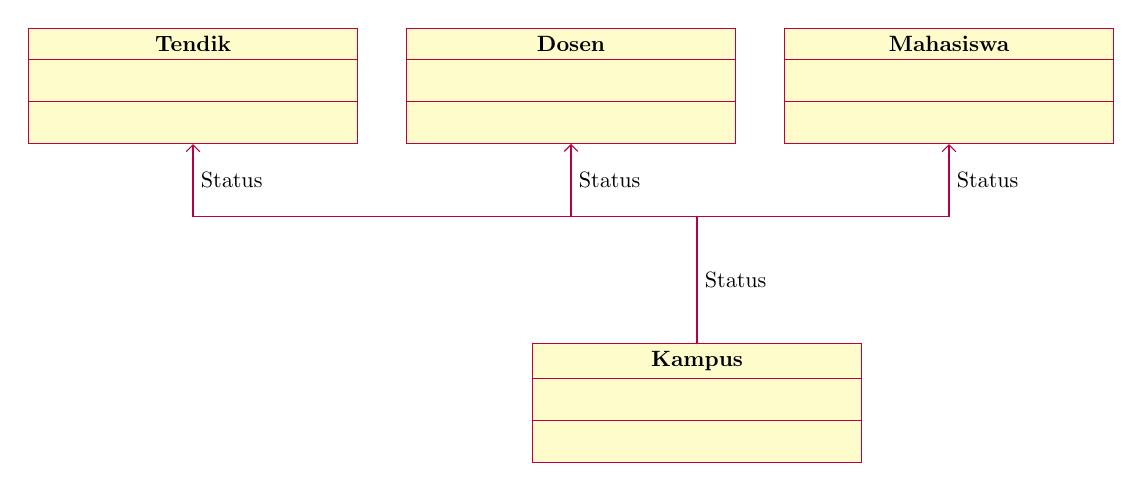
\begin{tikzpicture}[every node/.style={scale=1}, transform shape,scale=0.8]
        \begin{class}{Kampus}{0,0}
          \attribute{}
          \attribute{}
          \operation{}
          \operation{}
        \end{class}
      
        \begin{class}{Mahasiswa}{4,5}
          \attribute{}
          \attribute{}
          \operation{}
          \operation{}
        \end{class}
      
        \begin{class}{Dosen}{-2,5}
          \attribute{}
          \attribute{}
          \operation{}
          \operation{}
        \end{class}
      
        \begin{class}{Tendik}{-8,5}
          \attribute{}
          \attribute{}
          \operation{}
          \operation{}
        \end{class}
      
        \draw [umlcd style] (Kampus.north) -- ++(0,2cm)
                            coordinate (tmp)
                            node[right,midway] {Status};
      
        \foreach \endpoint in {Mahasiswa,Dosen,Tendik}
          \draw [umlcd style,fill=none,->] (tmp) -| (\endpoint.south)
                                           node[pos=0.75,right] {Status};
      \end{tikzpicture}
      \caption{Contoh Diagram UML sebagai gambaran dari pemrograman berorientasi objek}
    \end{figure}
  \end{frame}

  \begin{frame}
    \frametitle{\insertsection}
    \begin{figure}[h!]
      \centering
      
\includegraphics[width=0.4\textwidth]{soro soro jikanda}
    \end{figure}
    \begin{quote}
      ``Sekarang sudah waktunya untuk beralih dari \textit{Pemrograman Prosedural} ke \textit{Pemrograman Berorientasi Objek}.''
    \end{quote}
  \end{frame}

  \section{\textit{Class}}
  \begin{frame}[fragile]
    \frametitle{\insertsection}
    \begin{definisi}
      \textbf{Class} adalah template atau blueprint untuk membuat objek. Class mendefinisikan atribut (data) dan metode (fungsi) yang dimiliki oleh objek. Class adalah struktur data yang dapat digunakan untuk mengelompokkan data dan perilaku yang terkait.
    \end{definisi}
    \begin{lstlisting}[caption={Struktur Dasar Class}]
  class NamaClass {
    // Atribut (variabel)
    // Method (fungsi)
  }
    \end{lstlisting}
  \end{frame}

  \begin{frame}[fragile]
    \frametitle{\insertsection}
    \begin{block}{Atribut}
      Variabel yang dimiliki oleh class. Atribut dapat berupa variabel primitif (int, double, char, dll) atau objek dari class lain.
    \end{block}
    \begin{contoh}
      Mobil memiliki atribut seperti warna, merk, dan tahun keluaran.
    \end{contoh}
    \begin{lstlisting}[caption={Contoh Penambahan Atribut pada}]
    class Mobil {
      String merk;
      String warna;
      int tahun;
    }
    \end{lstlisting}
  \end{frame}

  \begin{frame}[fragile]
    \frametitle{\insertsection}
    \begin{block}{Method}
      Fungsi yang dimiliki oleh class. Method dapat berupa fungsi yang mengubah nilai atribut atau fungsi yang melakukan operasi tertentu.
    \end{block}
    \begin{contoh}
      Mobil memiliki method seperti mesin nyala dan mesin mati.
    \end{contoh}
    \begin{lstlisting}[caption={Contoh Penambahan Method pada Class Mobil}]
    class Mobil {
      //...
      void MesinModeAktifOn() {System.out.println("Mesin " + merk + " dinyalakan!");}
      void MesinModeNonaktifOff() {System.out.println("Mesin " + merk + " dimatikan!");}
    }
    \end{lstlisting}
  \end{frame}

  \subsection{\textit{Constructor}}
  \begin{frame}[fragile]
    \frametitle{\insertsection}
    \framesubtitle{\insertsubsection}
    \begin{definisi}
      \textbf{Constructor} adalah method khusus dalam class yang digunakan untuk menginisialisasi objek. Constructor memiliki nama yang sama dengan class dan tidak memiliki tipe pengembalian. Constructor dapat memiliki parameter untuk menginisialisasi atribut objek.
    \end{definisi}
    \begin{lstlisting}[caption={Struktur Constructor pada Class}]
    class NamaClass {
      Type atribut1, atribut2,...;
      NamaClass(Type param1, Type param2,...) { // Constructor
        this.atribut1 = param1;
        this.atribut2 = param2; 
        //...
      }
    }
    \end{lstlisting}
  \end{frame}

  \begin{frame}[fragile]
    \frametitle{\insertsection}
    \framesubtitle{\insertsubsection}
    \begin{lstlisting}[caption={Constructor pada Class Mobil}]
  class Mobil {
    String merk;
    String warna;
    int tahun;

    // Constructor
    Mobil(String merkInput, String warnaInput, int tahunInput) {
        this.merk = merkInput;
        this.warna = warnaInput;
        this.tahun = tahunInput;
    }
  }
    \end{lstlisting}
  \end{frame}

  \section{\textit{Object}}
  \begin{frame}[fragile]
    \frametitle{\insertsection}
    \begin{definisi}
      \textbf{Object} adalah instansiasi dari class. Object memiliki atribut dan metode yang didefinisikan dalam class. Setiap object memiliki nilai yang berbeda untuk atribut yang sama.
    \end{definisi}
    \begin{lstlisting}[caption={Contoh Instansiasi Object}]
    public static void main(String[] args) {
      NamaClass namaObject1 = new NamaClass();
      NamaClass namaObject2 = new NamaClass(parameter1, parameter2, ...);
    }
    \end{lstlisting}
  \end{frame}

  \begin{frame}[fragile]
    \frametitle{\insertsection}
    \begin{contoh}
      Contoh pembuatan objek mobil dan menggunakan perilakunya.
    \end{contoh}
    \begin{lstlisting}[caption={Contoh Penggunaan Object Mobil}]
    public static void main(String[] args) {
        Mobil mobilSaya = new Mobil(); // Membuat object
        Mobil mobilTeman = new Mobil("Esemka", "RGB", 2030); // Constructor
        
        mobilSaya.merk = "Toyota"; // Mengisi atribut
        mobilSaya.warna = "Putih";
        mobilSaya.tahun = 2020;

        mobilSaya.nyalakanMesin(); // Menggunakan method
        mobilSaya.matikanMesin();
    }
    \end{lstlisting}
  \end{frame}

  \section{Latihan}
  \begin{frame}
    \begin{latihan}
      Buatlah class \texttt{Mahasiswa} yang memiliki atribut sebagai berikut:
      \begin{multicols}{5}
        \begin{itemize}
          \item Nama
          \item NRP
          \item Jurusan
          \item TTL
          \item Tahun Masuk
          \item IPS
          \item IPK
          \item Alamat
          \item No HP
          \item Email
          \item Semester
          \item Status
        \end{itemize}
      \end{multicols}
      Kemudian buatlah beberapa method berikut:
        \begin{itemize}
          \item Menampilkam biodata diri
        \end{itemize}
    \end{latihan}
  \end{frame}
\end{document}